%% Sample latex file.
\documentclass[11pt]{article}

\usepackage{amsmath,amssymb,amsthm}
\usepackage{fullpage,times}
\usepackage{siunitx}
\usepackage{graphicx}
\usepackage{fancyhdr}
\usepackage{relsize}
\usepackage{hyperref}
\usepackage{indentfirst}

\renewcommand\qedsymbol{$\blacksquare$}

\title{Planar Point Location Problem with Persistent Search Trees}
\date{April 6, 2017}
\author{James Nhan (160149990)}

\begin{document}
\maketitle

\section{Introduction}
\label{sec:intro}

	The point location problem described by Neil Sarnak and Robert E. Tarjan in their paper "Planar point location using persistent search trees" \cite{sarnaktarjan} is one that takes a planar subdivision and a point. The goal is to determine which polygon the point resides in. Sarnak and Tarjan also detail using a specific type of data structure that is persistent across insertions and deletions. This enables a very fast query time while keeping size down. The associated program implements the solution described. A link to the GitHub repository can be found in at the end of the report.
	
\section{Program Description}
\label{sec:description}

	The program implements three main steps: constructing a doubly connected edge list (\texttt{DCEL}) from a simple polygon, monotonize and triangulate a simple polygon, and creating a \texttt{PointLocation} object using persistent red black trees. From that point, the user can then query the point location object with a \texttt{Point} object. This query will return the a half-edge that bounds the face containing the point. The program utilizes the sweep line method of creating a triangulated monotone polygon and the slab method to perform the point location query. This program utilizes an open source implementation of a persistent red black tree set by Tom Larkworthy \cite{tomlarkworthy} as described by Sarnak and Tarjan \cite{sarnaktarjan}.
	
\section{Features and Limitations}
\label{sec:featlims}

\subsection{Features}
\label{sec:features}

	The first main feature of the program is the implementation of a \texttt{DCEL} for describing the polygons. Begin with an array of \texttt{Point} objects. Each of which should represent a point of the polygon's outer boundary in counter-clockwise order. For some \texttt{DCEL} object, invoke its member method \texttt{ConstructSimplePolygon} method, passing in the array of \texttt{Point} objects. The \texttt{DCEL} object will contain the description of the polygon as a \texttt{HashSet} of \texttt{Face}, \texttt{HalfEdge}, and \texttt{Vertex} objects.
	
	Now, with a \texttt{DCEL}, we can monotonize it through its member method \texttt{MakeMonotone} and triangulate the resulting monotone polygon through another member method \texttt{TriangulateMonotonePolygon}.
	
	Finally, we may construct a \texttt{PointLocation} object. The constructor will take in a \texttt{DCEL} and construct a persistent red black tree set to contain slabs. This \texttt{PointLocation} object can then be used to query the planar subdivision with \texttt{Point} objects via the \texttt{Query} member method. The method is very fast. It can be done in $O\left( \log n \right)$ time. The size of the tree grows in $O\left( n \right)$ space due to the persistent nature of the tree and use of limited node copying. The description that Larkworthy provides mistakenly states that the size is $O\left( \log n \right)$.
	
\subsection{Limitations}
\label{sec:limitations}

	This program does have several limitations. It will not handle non-simple polygons. That is, any polygons with intersecting edges will fail to construct a simple polygon. In the event that \texttt{ConstructSimplePolygon} is invoked on a set of \texttt{Point} objects that define a polygon with intersecting points, an exception will be thrown.
	
	Another limitation stems from polygons with holes. Because the program defines the polygons via a list of points in counter-clockwise order, it is not possible to define a polygon with a hole; although, legacy code lingers to support it throughout. This limitation is confined to the construction of the polygon. Other parts of the program are not subject to this limitation with the exception of monotonizing and triangulating in the case of an edge going through a hole.
	
	Adding a \texttt{Vertex} to the polygon only works when adding one directly on an edge to split the edge; however, adding in the capability to add a vertex anywhere would not be difficult. We would simply have to get the two nearest vertices, add edges from them to the new \texttt{Vertex}, and finally, delete the edge between the two vertices.
	
	The polygon does contain a reference to the \texttt{Face} containing the polygon. That is, the \texttt{Face} that is unbounded on the outside. Should the point location query receive a \texttt{Point} that is within this \texttt{Face}, the query result will be \texttt{null}. If the user would like to instead retrieve a reference to the \texttt{Face} or \texttt{HalfEdge} bounding this face on the inside, a modification can be made in the \texttt{Query} method. Instead of returning \texttt{null} at the end, loop through the faces of the polygon and return the \texttt{Face} whose \texttt{GetInner()} object is \texttt{null}. This is the \texttt{Face} unbounded on the outside.
	
	To summarize the limitations, this program can only handle simple polygons that have no holes.
	
\section{Compiling and Running}
\label{compile}

	The original development environment of this project was in Eclipse Neon.3 Release (4.613). The build id is 20170314-1500. The JDK version used is 1.8.0\_91 and the JRE version targeted is 1.8.0\_91. Included in the GitHub repository are the Eclipse project files, and the project should compile and run out of the box.
	
	If the user wishes to compile and run via command line, the following command should be issued:
	
	\begin{center}
		\texttt{javac -d bin/ src/*.java}
	\end{center}
	
	\begin{center}
		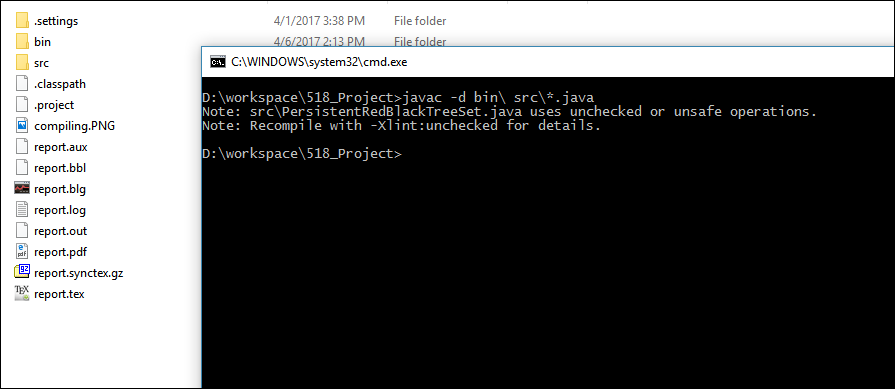
\includegraphics[scale=0.5]{compiling} \\
		\textbf{Figure 1}: Compiling the project.
	\end{center}
	
	To run from the command line, issue the command:
	
	\begin{center}
		\texttt{java -cp bin/ bin/Main}
	\end{center}
	
	\begin{center}
		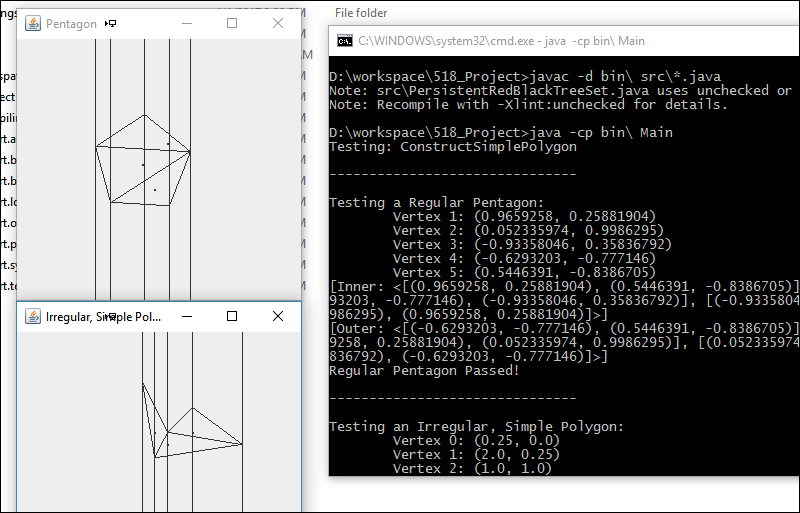
\includegraphics[scale=0.5]{running} \\
		\textbf{Figure 2}: Running the project.
	\end{center}
	
	The result will be the test output in the command line and two Swing windows to visualize the polygons, their triangulations, slabs, and points tested in the point location problem.
	
\section{API}
\label{sec:api}

\subsection{DCEL}
\label{sec:dcel}

	\texttt{DCEL()} - The default constructor. It will initialize an empty \texttt{DCEL} object.
	
	\texttt{AddEdge(Vertex, Vertex)} - Adds an edge between the two \texttt{Vertex} objects.
	
	\texttt{AddVertex(Vertex)} - Adds a \texttt{Vertex} to the polygon. The \texttt{Vertex} must be on an edge of the polygon.
	
	\texttt{ConstructSimplePolygon(Point[])} - Constructs a simple polygon from the \texttt{Point} array and stores it in the \texttt{DCEL}. Throws an exception for non-simple polygons.
	
	\texttt{GetEdge()} : \texttt{HashSet<HalfEdge>} - Returns the \texttt{HalfEdge} objects of the polygon.
	
	\texttt{GetFaces()} : \texttt{HashSet<Face>} - Returns the \texttt{Face} objects of the polygon.
	
	\texttt{GetVertices()} : \texttt{HashSet<Vertex>} - Returns the \texttt{Vertex} objects of the polygon.
	
	\texttt{IsSimplePolygon(Vertex[])} : \texttt{boolean} - Checks whether or not the \texttt{DCEL} is a simple polygon.
	
	\texttt{IsSimplePolygon(HashSet<Vertex>)} : \texttt{boolean} - Checks whether or not the \texttt{DCEL} is a simple polygon.

\subsection{Event}
\label{sec:event}

	\texttt{Event(HalfEdge, Vertex)} - The constructor. It will initialize an \texttt{Event} for the \texttt{Vertex} and the associated \texttt{HalfEdge}.
	
	\texttt{compareTo(Event)} : \texttt{int} - Compares the \texttt{Event} based on the incident \texttt{Vertex}.
	
	\texttt{GetEdge()} : \texttt{HalfEdge} - Returns the \texttt{HalfEdge} incident on the event point.
	
	\texttt{GetType()} - \texttt{EventType} - Gets the type of \texttt{Event} in the form of the \texttt{EventType} enum.
	
	\texttt{GetVertex()} : \texttt{Vertex} - Returns the \texttt{Vertex} incident on the event point.
	
	\texttt{SetEdge(HalfEdge)} - Sets the incident \texttt{HalfEdge}.
	
	\texttt{SetType(EventType)} - Sets the type of \texttt{Event} in the form of the \texttt{EventType} enum.
	
	\texttt{SetVertex(Vertex)} - Sets the incident \texttt{Vertex}.
	
\subsubsection{EventType}
\label{sec:eventtype}

	\texttt{LEFT} - An \texttt{Event} taking place on the left \texttt{Vertex} of an edge.
	
	\texttt{RIGHT} - An \texttt{Event} taking place on the right \texttt{Vertex} of an edge.

\subsection{EventQueue}
\label{sec:eventqueue}

	\texttt{EventQueue(Vertex[])} - The constructor. It will initialize an \texttt{EventQueue} for the \texttt{Vertex} array given with an \texttt{Event} for each \texttt{Vertex}.

\subsection{Face}
\label{sec:face}

	\texttt{Face()} - The default constructor. It will initialize an unbounded \texttt{Face}.
	
	\texttt{Face(HalfEdge, HalfEdge)} - The constructor. It will initialize a \texttt{Face} bounded on the outside by the first \texttt{HalfEdge} and with a single \texttt{HalfEdge} in the inside.
	
	\texttt{Face(HalfEdge, HashSet<HalfEdge>)} - The constructor. It will initialize a \texttt{Face} bounded on the outside by the first \texttt{HalfEdge} and holes defined by the \texttt{HashSet} of \texttt{HalfEdge} objects.
	
	\texttt{equals(Object)} : \texttt{boolean} - Compares whether or not two \texttt{Faces} are equivalent by comparing their boundaries and holes.
	
	\texttt{GetInner()} : \texttt{HashSet<HalfEdge>} - Returns the set of \texttt{HalfEdges} that form holes in the \texttt{Face}
	
	\texttt{GetOuter()} : \texttt{HalfEdge} - Returns a \texttt{HalfEdge} that bounds the \texttt{Face}.
	
	\texttt{hashCode()} : \texttt{int} - Returns a hash based on the hashes of the \texttt{HalfEdge} components of its outer boundary using a basic hash of prime numbers ($31$ and $17$).
	
	\texttt{IsConvex()} : \texttt{boolean} - Returns whether or not a \texttt{Face} is convex.
	
	\texttt{SetConvex(boolean)} - Sets the convex status of a \texttt{Face}.
	
	\texttt{SetInner(HashSet<HalfEdge>)} - Sets the set of \texttt{HalfEdge} objects that form holes in the \texttt{Face}.
	
	\texttt{SetOuter(HalfEdge)} - Sets the \texttt{HalfEdge} that bounds the \texttt{Face}.
	
	\texttt{toString()} : \texttt{String} - Returns a \texttt{String} representation of the \texttt{Face} as a list of its outer and inner boundaries.

\subsection{HalfEdge}
\label{sec:halfedge}

	\texttt{HalfEdge()} - The default constructor. It will initialize a \texttt{HalfEdge} with no endpoint or \texttt{Face}.
	
	\texttt{HalfEdge(HalfEdge)} - The copy constructor. It will initialize a \texttt{HalfEdge} with the same endpoints and bounded \texttt{Face} as the parameter.
	
	\texttt{HalfEdge(Vertex, Face, HalfEdge, HalfEdge, HalfEdge)} - The constructor. It will initialize a \texttt{HalfEdge} with an origin \texttt{Vertex}, a bounded \texttt{Face}, a next \texttt{HalfEdge}, a previous \texttt{HalfEdge}, and a twin \texttt{HalfEdge}.
	 
	\texttt{equals(Object)} : \texttt{boolean} - Compares whether or not two \texttt{HalfEdge} objects are equivalent by comparing their origins and their twins' origins.
	
	\texttt{GetDirection()} : \texttt{int} - Returns the direction of the \texttt{HalfEdge} chain. The results may be: $-1$ for counter-clockwise, $0$ for a single \texttt{HalfEdge}, or $1$ for clockwise.
	
	\texttt{GetFace()} : \texttt{Face} - Returns the \texttt{Face} bounded by the \texttt{HalfEdge} on the left.
	
	\texttt{GetHelper()} : \texttt{Vertex} - Returns the helper \texttt{Vertex} for triangulating a polygon.
	
	\texttt{GetNext()} : \texttt{HalfEdge} - Returns the next \texttt{HalfEdge} in the chain that bounds the same \texttt{Face}.
	
	\texttt{GetOrigin()} : \texttt{Vertex} - Returns the origin \texttt{Vertex} of the \texttt{HalfEdge}.
	
	\texttt{GetPrev()} : \texttt{HalfEdge} - Returns the previous \texttt{HalfEdge} in the chain that bounds the same \texttt{Face}.
	
	\texttt{GetTwin()} : \texttt{HalfEdge} - Returns the twin \texttt{HalfEdge} whose origin is the endpoint and whose endpoint is the origin of the current \texttt{HalfEdge}.
	
	\texttt{hashCode()} : \texttt{int} - Returns a hash based on the hashes of the \texttt{Vertex} components of its endpoints using a basic hash of prime numbers ($31$ and $17$).
	
	\texttt{SetFace(Face)} - Sets the incident \texttt{Face} on its left.
	
	\texttt{SetHelper(Vertex)} - Sets the helper \texttt{Vertex}.
	
	\texttt{SetNext(HalfEdge)} - Sets the next \texttt{HalfEdge} in the chain.
	
	\texttt{SetOrigin(Vertex)} - Sets the origin \texttt{Vertex} of the \texttt{HalfEdge}.
	
	\texttt{SetPrev(HalfEdge)} - Sets the previous \texttt{HalfEdge} in the chain.
	
	\texttt{SetTwin(HalfEdge)} - Sets the twin \texttt{HalfEdge}.
	
	\texttt{toString()} : \texttt{String} - Returns a \texttt{String} representation of the \texttt{HalfEdge} as a tuple of the endpoints.

\subsection{PersistentRedBlackTreeSet}
\label{sec:prbtree}

\texttt{PersistentRedBlackTreeSet<D>()} - The default constructor. It will initialize an \texttt{PersistentRedBlackTreeSet<D>} and use the default \texttt{Comparator} that compares via \texttt{hashCode}.

\texttt{PersistentRedBlackTreeSet<D>(Comparator<? super D>)} - The constructor. It will initialize a \texttt{PersistentRedBlackTreeSet<D>} and use the provided \texttt{Comparator<? super D>}.

\texttt{contains(Object)} : \texttt{boolean} - Returns whether or not the tree set contains an object.

\texttt{delete(D)} - Deletes an object from the tree set.

\texttt{equals(Object)} : \texttt{boolean} - Returns whether or not two trees are equivalent.
\texttt{get(D)} : \texttt{D} - Returns an element if it is in the tree set.

\texttt{getElements()} : \texttt{List<D>} - Returns a \texttt{List} of all of the elements in the tree set sorted in-order traversal.

\texttt{getRandomLeaf()} : \texttt{D} - Returns a random leaf element in the list in $O\left( \log n \right)$ time. Some elements are not stored in leaves, so they will not be sampled.

\texttt{GetRootNode()} : \texttt{RedBlackNode<D>} - Returns the root node of the tree set.

\texttt{hashCode()} : \texttt{int} - Returns the hash of the tree.

\texttt{insert(D)} : \texttt{PersistentRedBlackTreeSet<D>} - Returns the tree with the new data element. The original list remains the same. This is a persistent insertion.

\texttt{insertSubTree(PersistentRedBlackTreeSet<D>)} : \texttt{PersistentRedBlackTreeSet<D>} - Returns the tree with the subtree inserted persistently. All subelements of the subtree remain in the same order. use with caution.

\texttt{iterator()} : \texttt{Iterator<D>} - Returns an iterator of the tree for in-order traversal over all of the elements in the tree.

\texttt{size()} : \texttt{int} - Returns the number of elements inserted in the tree.

\subsubsection{RedBlackTreeNode}
\label{sec:node}

\texttt{RedBlackNode<D>()} - The default constructor. It will initialize a \texttt{RedBlackNode<D>} with no element or children. Its color will be \texttt{null}.

\texttt{RedBlackNode<D>(D)} - The constructor. It will initialize a red \texttt{RedBlackNode<D>} with a specific element. Its children will be black \texttt{null} nodes.

\texttt{RedBlackNode<D>(RedBlackNode<D>)} - The child constructor. It will initialize a black \texttt{RedBlackNode<D>} with no element.

\texttt{clone()} : \texttt{RedBlackNode<D>} - Returns a shallow clone of the parameter.

\texttt{cloneSibling(LinkedList<RedBlackNode<D>>)} - Clones the sibling where the parameter is the list of nodes above in the tree.

\texttt{cloneUncle(LinkedList<RedBlackNode<D>>)}  - Clones the uncle where the parameter is the list of nodes above in the tree.

\texttt{deepClone()} : \texttt{RedBlackNode<D>} - Returns a deep clone of the parameter.

\texttt{GetElement()} : \texttt{D} - Returns the element in the node.

\texttt{GetLeft()}  : \texttt{RedBlackNode<D>} - Returns the left child of the node.

\texttt{GetRight()} : \texttt{RedBlackNode<D>} - Returns the right child of the node.

\texttt{sibling(LinkedList<RedBlackNode<D>>)} : \texttt{RedBlackNode<D>} - Returns the sibling of the node where the parameter is the list of nodes above in the tree.

\subsection{Point}
\label{sec:point}

\texttt{Point(float, float)} - The constructor. It will initialize a \texttt{Point} at the given x-y coordinates.

\texttt{Cross(Point, Point, Point)} : \texttt{float} - Returns the cross product of the lines extending from the first \texttt{Point} object to the other two.

\texttt{Dot(Point, Point)}  : \texttt{float} - Returns the dot product of the two \texttt{Point} objects.

\texttt{Dot(Point, Point, Point)} : \texttt{float} - Returns the dot product of the lines extending from the first \texttt{Point} object to the other two.

\texttt{compareTo(Point)} : \texttt{int} - Returns the relative location of the parameter \texttt{Point} object. The possible return values are: $-1$ is the parameter is to the right or above, $0$ if the parameter is at the same location, $1$ if the parameter is to the left or below.

\texttt{equals(Object)} : \texttt{boolean} - Returns whether or not the two \texttt{Point} objects are equivalent.

\texttt{GetX()} : \texttt{float} - Returns the x-coordinate.

\texttt{GetY()} : \texttt{float} - Returns the y-coordinate.

\texttt{hashCode()} : \texttt{int} - Returns the hash of the \texttt{Point} based on a counter system.

\texttt{IsBetween(Point, Point)} : \texttt{boolean} - Returns whether or not this \texttt{Point} is collinear with the parameters.

\texttt{IsLeft(HalfEdge)} : \texttt{boolean} - Returns whether or not this \texttt{Point} is to the left of a \texttt{HalfEdge}.

\texttt{SetX(float)} - Sets the x-coordinate of the \texttt{Point}.

\texttt{SetY(float)} - Sets the y-coordinate of the \texttt{Point}.

\texttt{toString()} - Returns a \texttt{String} representation of the \texttt{Point} as a tuple of the x-y coordinates.

\subsection{PointLocation}
\label{sec:pointlocation}

\texttt{PointLocation(DCEL)} - The constructor. It will initialize a \texttt{PointLocation} structure for the associated \texttt{DCEL}.

\texttt{GetSlabs()} : \texttt{List<Slab>} - Returns the \texttt{Slab} objects of the \texttt{PointLocation} structure generated.
 
\texttt{Query(Point)} : \texttt{HalfEdge} - Returns a \texttt{HalfEdge} that bounds the \texttt{Face} that contains the \texttt{Point}. Returns \texttt{null} if the \texttt{Point} is not within any internal \texttt{Face} of the \texttt{DCEL}.

\subsection{Slab}
\label{sec:slab}

\texttt{Slab(Point, Point)} - The constructor. It will initialize a \texttt{Slab} that has a left bound and right bound.

\texttt{AddEdge(HalfEdge)} - Adds a \texttt{HalfEdge} to the \texttt{Slab}.

\texttt{GetEdgeBelow(Point)} : \texttt{HalfEdge} - Returns the \texttt{HalfEdge} directly below the \texttt{Point}.

\texttt{GetLeftBound()} : \texttt{Point} - Returns the left bound of the \texttt{Slab}.

\texttt{GetRightBound()} : \texttt{Point} - Returns the right bound of the \texttt{Slab}.

\texttt{IsInSlab(Point)} : \texttt{boolean} - Returns whether or not a \texttt{Point} is within the bounds of the \texttt{Slab}.

\subsection{SweepLine}
\label{sec:sweepline}

\texttt{SweepLine()} - The default constructor. It will initialize a \texttt{SweepLine} with a no \texttt{Segments}.

\texttt{AddEvent(Event)} : \texttt{Segment} - Adds an \texttt{Event} to the \texttt{SweepLine} and returns its corresponding \texttt{Segment}.

\texttt{FindEvent(Event)} : \texttt{Segment} - Returns the \texttt{Segment} that corresponds to the \texttt{Event}.

\texttt{Intersect(Segment, Segment)} : \texttt{boolean} - Returns whether or not the two \texttt{Segment} objects intersect.

\texttt{RemoveSegment(Segment)} - Removes a \texttt{Segment} from the \texttt{SweepLine}.

\subsubsection{Segment}
\label{sec:segment}

\texttt{compareTo(Segment)} : \texttt{int} - Returns the relative position of the parameter. The possible return values are: $-1$ if the parameter is below, $0$ if the parameter is the same, $1$ if the parameter is above.

\texttt{equals(Object)} : \texttt{boolean} - Returns whether or not the two \texttt{Segment} objects are equivalent.

\texttt{GetAbove()} : \texttt{Segment} - Returns the \texttt{Segment} directly above it.

\texttt{GetBelow()} : \texttt{Segment} - Returns the \texttt{Segment} directly below it.

\texttt{GetEdge()} : \texttt{HalfEdge} - Returns the \texttt{HalfEdge} corresponding to this \texttt{Segment}.

\texttt{GetLeftVertex()} : \texttt{Vertex} - Returns the left endpoint.

\texttt{GetRightVertex()} : \texttt{Vertex} - Returns the left endpoint.

\texttt{hashCode()} : \texttt{int} - Returns the hash of the corresponding \texttt{HalfEdge}.

\texttt{SetAbove(Segment)} - Sets the \texttt{Segment} directly above it.

\texttt{SetBelow(Segment)} - Sets the \texttt{Segment} directly below it.

\texttt{SetEdge(HalfEdge)} - Sets the \texttt{HalfEdge} corresponding to this \texttt{Segment}.

\texttt{SetLeftVertex(Vertex)} - Sets the left endpoint.

\texttt{SetRightVertex(Vertex)} - Sets the left endpoint.

\subsection{Triangulation}
\label{sec:triangulation}

\texttt{IsMonotonePolygon(DCEL)} : \texttt{boolean} - Returns whether or not a \texttt{DCEL} is a monotone polygon.

\texttt{MakeMonotone(DCEL)} - Adds \texttt{HalfEdges} to the simple \texttt{DCEL} to make a monotone polygon.

\texttt{TriangulateMonotonePolygon(DCEL)} - Adds \texttt{HalfEdges} to the monotone \texttt{DCEL} to make a triangulated monotone polygon.

\subsection{Vertex}
\label{sec:vertex}

\texttt{Vertex()} - The default constructor. It will initialize a \texttt{Vertex} with no point, incident edge, \texttt{UNKNOWN} type, and non-convex.

\texttt{Vertex(Point)} - A constructor. It will initialize a \texttt{Vertex} with a point, but no incident edge, \texttt{UNKNOWN} type, and non-convex.

\texttt{Vertex(Point, HalfEdge)} - A constructor. It will initialize a \texttt{Vertex} with a point and incident edge, but with \texttt{UNKNOWN} type and non-convex.

\texttt{compareTo(Vertex)} : \texttt{int} - Returns the \texttt{compareTo} result of the two \texttt{Points}.

\texttt{equals(Object)} : \texttt{boolean} - Returns whether or not two \texttt{Vertex} objects are equivalent.

\texttt{GetEdge()} : \texttt{HalfEdge} - Returns one of the \texttt{HalfEdge} incident on this \texttt{Vertex}.

\texttt{GetPoint()} : \texttt{Point} - Returns the \texttt{Point} object of this \texttt{Vertex}.

\texttt{GetType()} : \texttt{Type} - Returns the \texttt{Type} of this \texttt{Vertex} for triangulation.

\texttt{hashCode()} : \texttt{int} - Returns the hash of the \texttt{Point}.

\texttt{IsConvex()} : \texttt{boolean} - Returns  whether or not this \texttt{Vertex} is convex.

\texttt{SetConvex(boolean)} - Sets the convex status of this \texttt{Vertex}.

\texttt{SetEdge(HalfEdge)} - Sets the incident edge of this \texttt{Vertex}.

\texttt{SetPoint(Point)} - Sets the location of this \texttt{Vertex}.

\texttt{SetType(Type)} - Sets the \texttt{Type} of this \texttt{Vertex}.

\texttt{toString()} - Returns the \texttt{String} representation of this \texttt{Vertex} as the tuple of the x-y coordinates.

\subsubsection{Type}
\label{sec:verttype}

\texttt{START} - A start \texttt{Vertex}.

\texttt{END} - An end \texttt{Vertex}.

\texttt{MERGE} - A merge \texttt{Vertex}.

\texttt{SPLIT} - A split \texttt{Vertex}.

\texttt{REGULARL} - A regular \texttt{Vertex} in the left chain.

\texttt{REGULARR} - A regular \texttt{Vertex} in the right chain.

\texttt{UNKNOWN} - An uncategorized \texttt{Vertex}.

\begin{thebibliography}{9}
	\bibitem{sarnaktarjan}
	Sarnak, Neil; Tarjan, Robert E.
	\textit{Point location problem with persistent search trees}
	
	\bibitem{tomlarkworthy}
	Larkworthy, Tom.
	\textit{PersistentRedBlackTreeSet}
	\url{https://edinburghhacklab.com/2011/07/a-java-implementation-of-persistent-red-black-trees-open-sourced/}
\end{thebibliography}

\end{document}
